%%%%%%%%%%%%%%%%%%%%%%%%%%%%%%%%%%%%%%%%%%%%%%%%%%%%%%%%%%%%%%%%%%%%%%%%%
% CHAPTER SpDCache
%%%%%%%%%%%%%%%%%%%%%%%%%%%%%%%%%%%%%%%%%%%%%%%%%%%%%%%%%%%%%%%%%%%%%%%%%

\chapter[SpDCache]{SpDCache}
\label{cha:spdc}

\minitoc

% \input{}



%%%%%%%%%%%%%
%%from ASAP

%%red cache and op spmv behavior
% Performing a \emph{reduction} in hardware requires a \emph{READ} from memory,
% followed by an accumulation and a \emph{WRITE} back. This operation is denoted
% $\mathit{RED}(key, value)$~\cite{Srikanth2021_SortCache} with the \emph{key} being
% the position in the output vector $c$.
% In Fig.~\ref{fig:GC_cache_WB}, we show three cases that occur in a generic data cache when a
% \emph{reduction} is performed. If the vector entry ($c_{key}$) 
% \emph{hits} in the cache, the \emph{update} is performed by the processor
% with no external memory access.
% When there is a \emph{miss}, the operation is blocked until 
% the \emph{READ} from main memory completes. Potentially, the \emph{miss} will also 
% trigger an \emph{eviction}, which exacerbates the blocking condition, because
% a cache-line must first be written back, before the \emph{READ} from main memory can 
% be performed. In scientific applications, the matrices are extremely
% large and only a small portion of the vector $c$ can reside in the cache, thus
% the \emph{miss+evict} case arises frequently.

% A \emph{reduction cache}, such as~\cite{Srikanth2021_SortCache} or~\cite{Mukkara2019_PHI},
% is a data-cache which accepts
% \emph{reduction} instructions (\emph{RED}) from the processor and performs accumulations locally (near-memory).
% In the case of a \emph{hit}, see Fig.~\ref{fig:red_based_cache}, the \emph{reduction}
% takes place in the cache. For a \emph{miss}, the cache allocates a new line
% with zeros, and simply inserts the value. In this case,
% the cache-line is inconsistent with main memory. Only when the line needs to be evicted,
% is a \emph{READ} performed. In the cache, the values in the line are accumulated with the main memory data, and the result
% is written back. As seen in the figure, a \emph{reduction cache} reduces the number
% of main memory accesses in the case of a \emph{miss}. At the end of the algorithm, the cache
% must be flushed.

% \begin{figure}[htbp]
%     \centering
%     \begin{subfigure}[t]{0.506493506\linewidth} %39/77 (39/73)
%         \centering
%         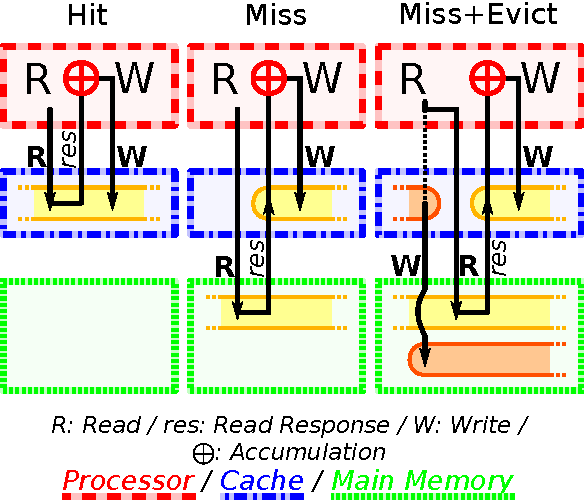
\includegraphics[width=\linewidth]{Figures/PDF/HardwareSpecs_RWtransactions_1.pdf}
%         \caption{Generic Cache (Write-Back)}
%         \label{fig:GC_cache_WB}
%     \end{subfigure}
%     \hfill
%     \begin{subfigure}[t]{0.441558442\linewidth} %34/77 (34/73)
%         \centering
%         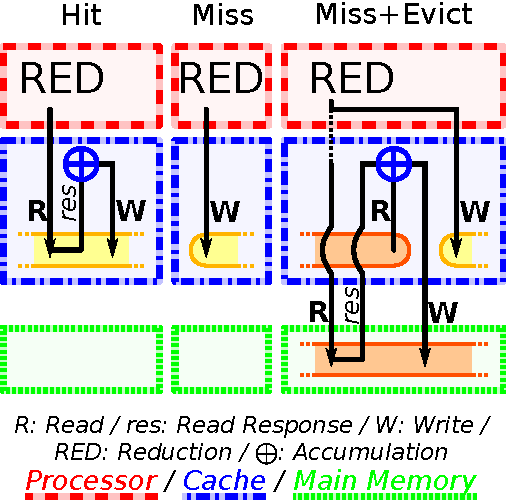
\includegraphics[width=\linewidth]{Figures/PDF/HardwareSpecs_RWtransactions_2.pdf}
%         \caption{Reduction Cache}
%         \label{fig:red_based_cache}
%     \end{subfigure}
%     \caption{\emph{READ} and \emph{WRITE} Transactions of a \emph{Reduction} Operation in Generic and \emph{Reduction} Caches}
%     \label{fig:RWtransactions}
% \end{figure}

% A widely used \emph{sparse format} to compress the non-zero elements in the matrix $A$ is \emph{CSC} (\emph{Compressed Sparse Column})~\cite{Saad2003_COO_CSR_DIA_ELL},
% where $A$ is a sparse matrix of dimensions $(M, N)$ with a number of non-zero elements $\mathit{NNZ}$. 
% It consists of three tables ($\mathit{VAL}$, $\mathit{IDX}$, $\mathit{PTR}$) used to store non-zero values, row indices and column positions.
% When performing an \algo{OP} SpMV ($A.b = c$) with this format (Algorithm~\ref{alg:spmv_with_red}),
% we see that a \emph{RED} is needed to accumulate the output vector $c$ (line~6). Moreover, $A$ is read sequentially 
% while $c$ is updated ``randomly''.
% In fact, the \emph{key} is determined via an indirection with an access to $\mathit{IDX}$.

% \begin{algorithm}[htbp]
%     \def\_{\!\!\!\!\!\!}
%     \caption{\emph{Outer-Product} SpMV -- Single Threaded}\label{alg:spmv_with_red}
%     \For(\Comment*[f]{\_ loop \_ over \_ columns \_ of \_ A \_}){$n \in \ldb 0, N-1 \rdb$}{
%         $\mathit{currPos}, \mathit{nextPos} \gets \mathit{PTR}_n, \mathit{PTR}_{n+1}$\;
%         \For{$pos \in \ldb \mathit{currPos}, \mathit{nextPos}-1 \rdb$}{
%             $key \gets \mathit{IDX}_{pos}$\Comment*[r]{\_ row \_ index \_}
%             $val \gets \mathit{VAL}_{pos} \times b_n$\Comment*[r]{\_ val \_ = \_ A\textsubscript{key,n} \_ $\times$ \_ b\textsubscript{n} \_}
%             $\mathit{RED}(key, val)$\Comment*[r]{\_ c\textsubscript{key} \_ += \_ val \_}
%         }
%     }
% \end{algorithm}

% In memory, $A$ is stored as three dense tables, but conceptually, as we perform
% the \algo{OP} multiplication, the matrix is traversed from top to bottom, then left to right. A row
% in the matrix corresponds to a \emph{key}, or equivalently, a position in the output vector $c$. In
% Fig.~\ref{fig:spmv_on_matrix}, we show an example of a sparse matrix with a few non-zero values
% (\ding{192} - \ding{197}). 
% As we traverse the matrix, we first perform a \emph{reduction} for the value on row $\mathit{key}_{10}$,
% then on row $\mathit{key}_{20}$ and then $\mathit{key}_{30}$. Each of these results in a 
% \emph{RED} on $c$. As we continue, we then \emph{hit} another
% value \ding{196} on the row $\mathit{key}_{10}$ which must be \emph{reduced} with an existing entry \ding{192}
% (as shown on the left of Fig.~\ref{fig:spmv_on_matrix}, \emph{Conceptual View}).

% \begin{figure}[htbp]
%     \centering
%     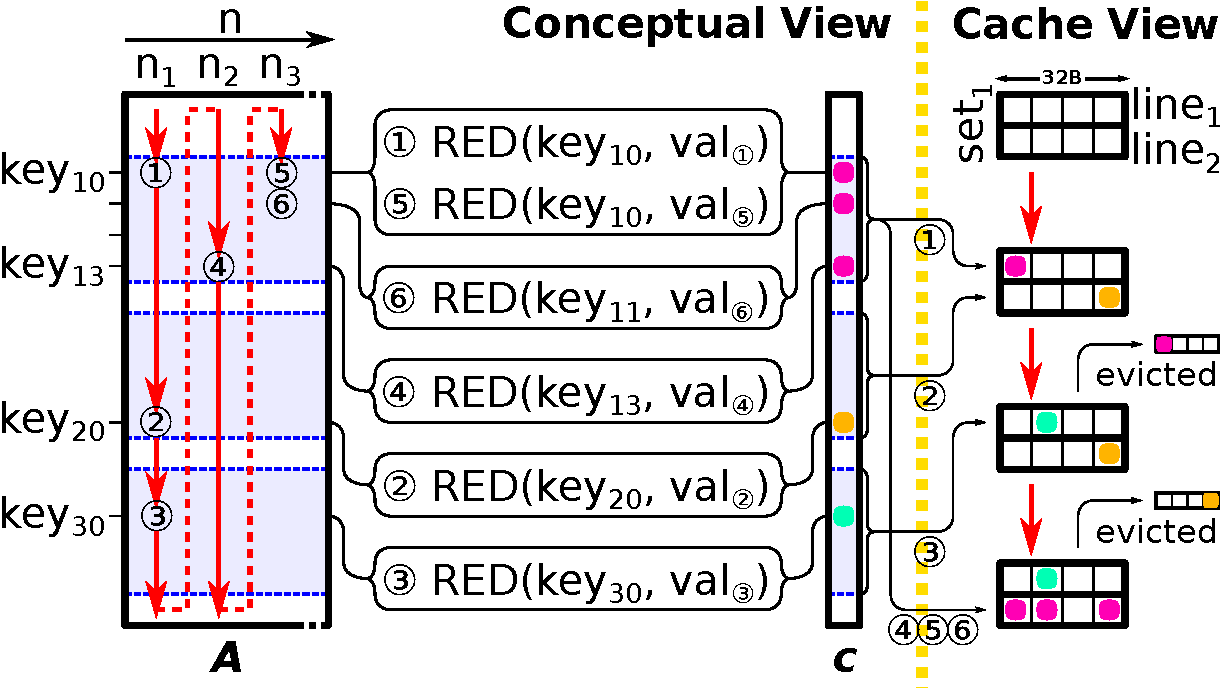
\includegraphics[width=1\linewidth]{Figures/PDF/HardwareSpecs_SpMVonMatrix.pdf}
%     \caption{Traversal of Non-Zero Elements of Input Matrix for \algo{OP} SpMV (left) and Impact on Cache (right)}
%     \label{fig:spmv_on_matrix}
% \end{figure}

% Let us consider how $c$ is stored in a two-way set-associative cache with 32B lines.
% We assume that all the \emph{keys} map to $\mathit{set}_1$.
% When \ding{192} is updated, there is a \emph{miss} and $\mathit{line}_1$ is allocated for $\mathit{key}_{10}$.
% Similarly with \ding{193}, $\mathit{line}_2$ is allocated for $\mathit{key}_{20}$.
% When $\mathit{key}_{30}$ comes along, an \emph{eviction} must be performed. We assume $\mathit{line}_1$, holding $\mathit{key}_{10}$,
% is evicted. We then come to \ding{195} which has $\mathit{key}_{13}$, adjacent in memory to $\mathit{key}_{10}$,
% and thus stored in the same line. This line must be brought back to process \mbox{\ding{195} - \ding{197}}.

% This example illustrates how a conventional cache can be inefficient.
% First, we note the line holding $\mathit{key}_{10}$ was evicted, although it
% was frequently accessed after \ding{192}. This \emph{eviction} was triggered by $\mathit{key}_{30}$, which was only accessed once. 
% Furthermore, for $\mathit{key}_{20}$ and $\mathit{key}_{30}$, a full line was loaded, only to 
% modify a single entry. A ``smarter'' cache would have maintained the line with $\mathit{key}_{10}$ 
% to avoid an unnecessary main memory access. Furthermore, this ``smarter'' cache would not have
% allocated full lines for $\mathit{key}_{20}$ and $\mathit{key}_{30}$ to only modify a single word.
% In the following sections, we explain how SpDCache achieves these ``smart'' behavior.

%%archi SpDC
% As shown in Fig.~\ref{fig:cache_partition}, SpDCache is divided into three regions\footnote{SpDCache could be implemented as a mode of a generic cache.}. The first, \emph{GRC} (\emph{Generic Region Cache}), is 
% for all memory transactions unrelated to the output vector $c$, including reads of $A$ and $b$.
% It is a classic, set-associative cache and not our focus, but is required for the processor to operate normally.
% The other two regions, called \emph{IBRC} and \emph{OBRT}, are able to perform \emph{reductions} on $c$.
% The \emph{IBRC} works as a line-wise, set-associative \emph{reduction cache} to hold high density data in the \emph{IBR}.
% The difference with the \emph{GRC} is that it
% is able to perform \emph{reductions} and it is dedicated to the \emph{banded} region, so that spurious accesses do not provoke undesired \emph{evictions}.
% Finally, the \emph{OBRT} works as an element-wise, fully-associative table whose role is to handle sparse regions (\emph{OBR}).

% \vspace{-5mm}
% \begin{figure}[htbp]
%     \centering
%     \begin{minipage}[b]{0.58\linewidth}
%         \begin{figure}[H]
%     		\centering
%     		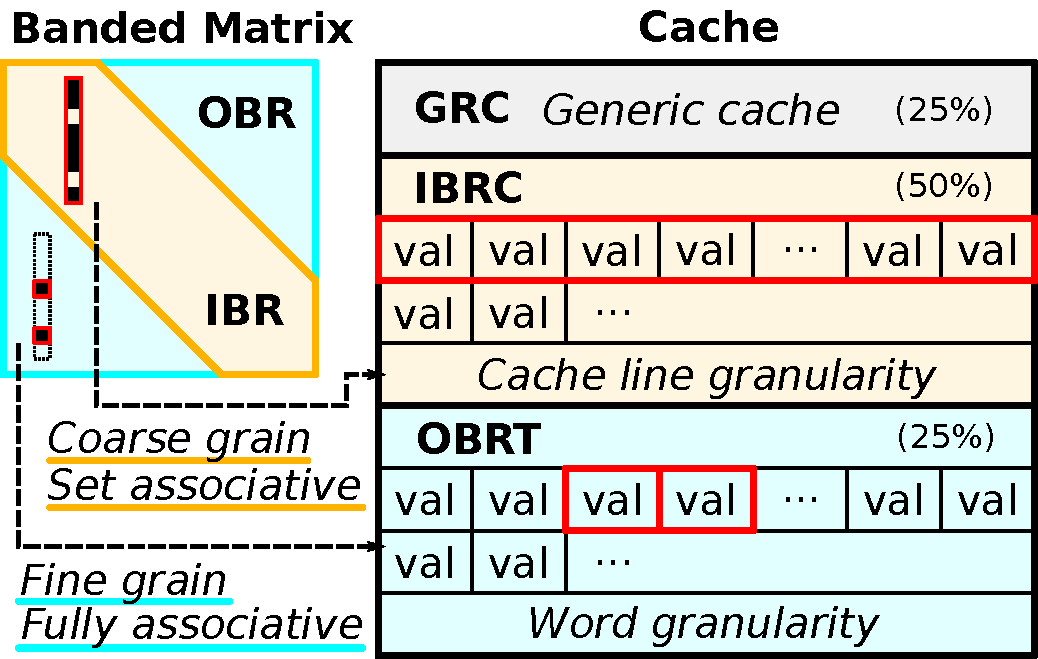
\includegraphics[width=\linewidth]{Figures/PDF/HardwareSpecs_MatrixAndDataCachePartition.pdf}
%     		\caption{Data-Cache Partitioning into Regions (GRC, IBRC, OBRT)}
%     		\label{fig:cache_partition}
%     	\end{figure}
%     \end{minipage}
%     \hfill
%     \begin{minipage}[b]{0.38\linewidth}
%     	\begin{figure}[H]
%     		\centering
%     		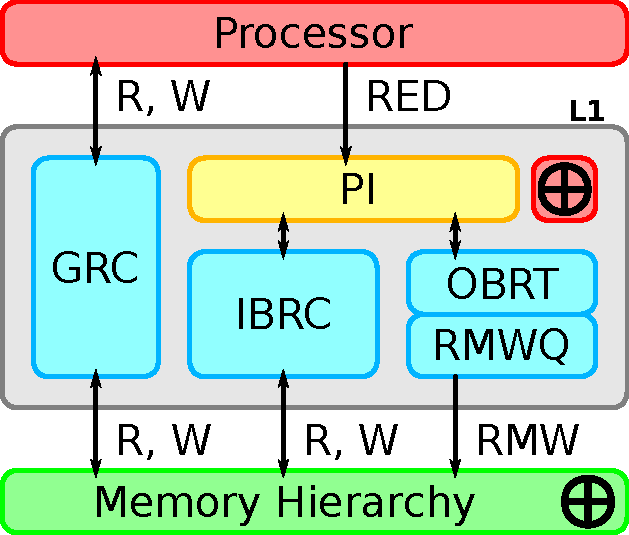
\includegraphics[width=\linewidth]{Figures/PDF/HardwareSpecs_GlobalViewArchi_Simplified.pdf}
%     		\caption{Simplified View of the Memory Hierarchy with SpDCache}
%     		\label{fig:global_view_archi}
%     	\end{figure}
%     \end{minipage}
% \end{figure}

% Fig.~\ref{fig:global_view_archi} shows a simplified view of a memory hierarchy with SpDCache. The \emph{Processor Interface} (\emph{PI}) takes
% \emph{reduction} operations, \emph{RED(key, value, region)}, from the processor and dispatches them to the \emph{IBRC} and \emph{OBRT}, depending on the \emph{region} argument.
% The \emph{IBRC} communicates with the memory hierarchy using \emph{READ} and \emph{WRITE} transactions over entire cache-lines, to propagate the local \emph{updates}
% to the downstream memory.
% As \emph{OBRT} \emph{updates} are for isolated elements, it does not make sense to bring a full line into the L1 to modify a 
% single word. 
% The \emph{OBRT} thus propagates \emph{updates} by issuing atomic Read-Modify-Write transactions (\emph{RMWs}), which must be processed remotely and 
% close to the main memory. 
% Existing protocols such as \mbox{AXI-4}~\cite{ARM2023_AXI} already support atomic transactions for certain operations (logical, integer add, min, max) and
% these would need to be extended to include floating point addition.
% The \emph{RMWs} from the \emph{OBRT} are temporarily buffered in a small queue (\emph{RMWQ}), to avoid congestion.

% SpDCache is driven by three key design principles.
% First, we ensure a given \emph{key} is in only one region, to avoid coherency problems.
% Second, the \emph{IBRC} is given priority over the \emph{OBRT}, to enable coalescing.
% Third, we avoid bringing a full line from memory to the L1 to simply update a few entries.

% \begin{figure}[htbp]
%     \centering
%     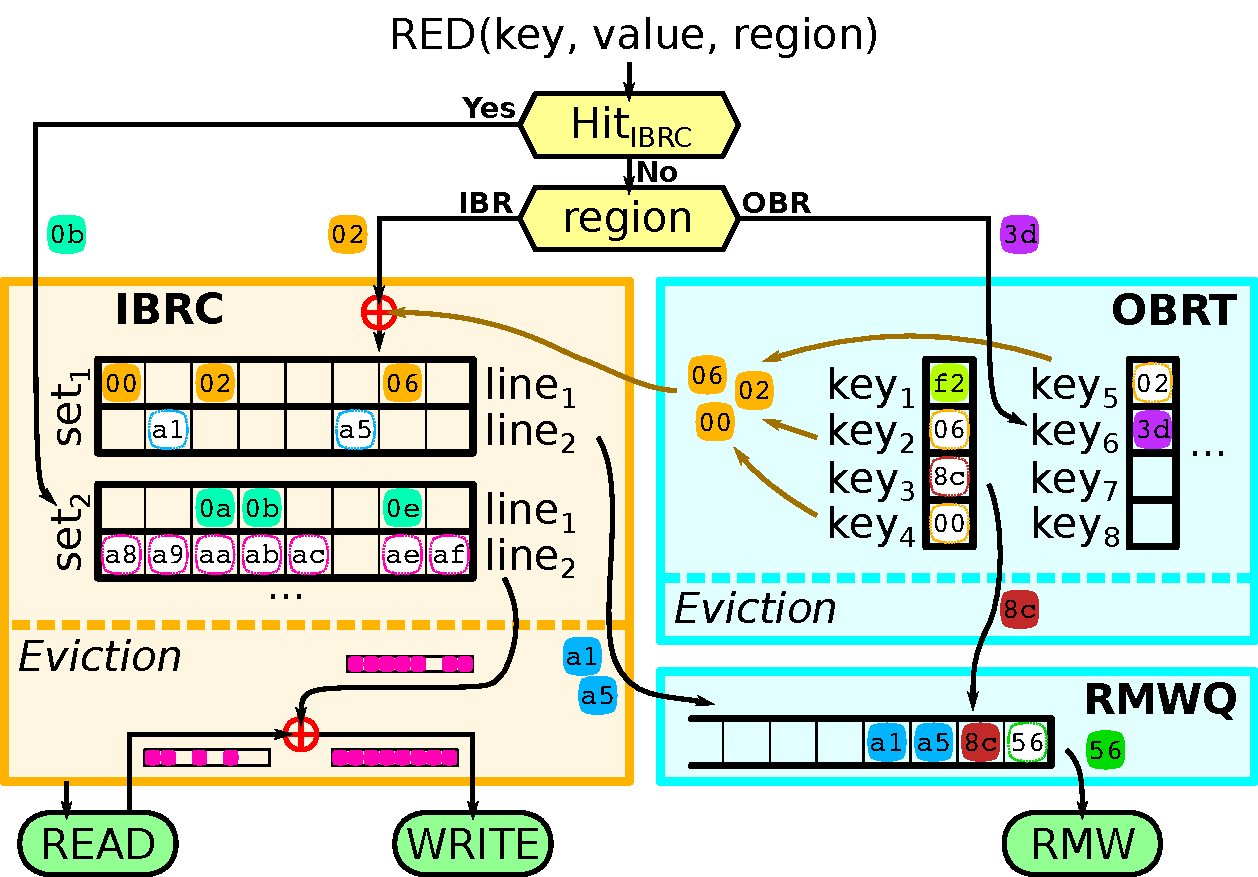
\includegraphics[width=1\linewidth]{Figures/PDF/HardwareSpecs_SpDC_behavior.pdf}
%     \caption{Internal Operation of SpDCache with Examples} % Internal Operation of SpDCache
%     \label{fig:spdc_archi}
% \end{figure}

% In Fig.~\ref{fig:spdc_archi}, we describe the operation of SpDCache, 
% via a series of scenarios, each shown in a different color.
% When a new \emph{reduction} \emph{RED(key, value, region)} is received from the processor, 
% we test for a \emph{hit} in the \emph{IBRC}, regardless of the \emph{region} argument.
% If it \emph{hits}, the value (case \addr{0b} -- \textit{turquoise}) can be accumulated in 
% the corresponding line of the \emph{IBRC}. We give this priority to the \emph{IBRC} as
% part of the mechanism to avoid duplication.

% If there is a \emph{miss} in the \emph{IBRC}, then the target region is 
% determined based on the \emph{region} argument of the \emph{RED} transaction.
% If it is \emph{IBR}, then it
% is necessarily a \emph{miss} case, and the value (\addr{02} -- \textit{orange}) must be inserted into a free cache-line of 
% the \emph{IBRC}. When we allocate this line, we ensure that it does not create
% a duplication of existing entries in the \emph{OBRT}. If there is duplication, as in
% our example, these entries (\addr{00}, \addr{02}, \addr{06}) are deleted from
% the \emph{OBRT} and merged into the newly allocated line ($set_1, line_1$).

% If the target region is the \emph{OBR}, then the \emph{reduction} (\addr{3d} -- \textit{purple})
% is processed in the \emph{OBRT}, either allocating a new entry (\emph{miss} case) or accumulating with 
% an existing entry (\emph{hit} case).

% Now, we describe the \emph{eviction} scenarios. In the \emph{IBRC}, the line to evict is selected
% ($set_2, line_2$ -- \textit{pink}), a \emph{READ} to main memory is performed, the values from
% the evicted line are accumulated and a \emph{WRITE} to main memory is issued.
% If the evicted line only has a few
% non-zero elements, it is a special case. To avoid bringing a full line
% from main memory, the non-zero values (\addr{a1} and \addr{a5} -- \textit{blue}) are 
% converted to atomic \emph{RMWs} and pushed onto the \emph{RMWQ}.

% The width of the \emph{band} ($W_B$), must be selected so that one column of the \emph{band}
% remains blocked in the \emph{IBRC}, otherwise, this region of the cache is
% always thrashing. This is our approach to selecting $W_B$ and it is independent of the matrix.

% In the \emph{OBRT}, an \emph{eviction} simply consists of moving the element from the table to the 
% \emph{RMWQ} (\addr{8c} -- \textit{brown}).
% \emph{OBRT} \emph{evictions} are issued in advance when the table is nearly full.
% The \emph{RMWQ} issues atomic \emph{RMWs} when it is not empty (\addr{56} -- \textit{dark green}).


%%experimental results
% We modeled the behavior of SpDCache (based on the flowchart in Fig.~\ref{fig:spdc_archi}) using a transaction-level model in Python, for a single-core, 
% single-thread system executing a \algo{OP} SpMV kernel (Algorithm~\ref{alg:spmv_with_red}).
% We do not model timing, as the order of the memory accesses determines the behavior of the cache
% (\emph{hits}, \emph{misses}, \emph{evictions}), which depends only on the SpMV algorithm.
% The model checks the final numerical result and reports the main memory traffic associated with 
% the \emph{updates} to the output vector (\emph{Output Memory Traffic}), where 
% we count the bytes transferred (64B for each \emph{READ} and \emph{WRITE}, and 8B per atomic \emph{RMW}, 
% with our configuration). For each \emph{WRITE} transaction, it tracks how many words in the line 
% were actually used (\emph{Evicted Cache Line Utilization}) and it tracks how many 
% words in the cache held useful data (\emph{Cache Memory Utilization}). We consider a word 
% in the cache to be useful if it is updated or inserted by the processor.
% Our goal is to validate the principle of SpDCache using real application matrices 
% from SuiteSparse Matrix Collection~\cite{Kolodziej2019_SuiteSparse}.

% As baselines, we implemented a fully generic cache (GC) that handle \emph{READs} and \emph{WRITEs} for both 
% inputs ($A$, $b$) and output ($c$), following the data movements shown in Fig.~\ref{fig:GC_cache_WB}, and 
% a simple \emph{reduction cache} (RedC) that processes \emph{RED} transactions in a dedicated region 
% using the flow shown in Fig.~\ref{fig:red_based_cache}.
% In the RedC, 25\% of the memory is allocated for the inputs and the other 75\% for \emph{REDs} on $c$.
% In SpDCache (SpDC), 25\% is allocated for the \emph{GRC}, 50\% for the \emph{IBRC}
% and 25\% for the \emph{OBRT}.
% All three caches use a \emph{random} eviction policy and have a total data storage of 32~kiB, and we do not account
% for the \emph{TAG} storage. The set associative regions have 4~ways 
% and 64B cache lines (8 \emph{double} words per line).

% We simulated 48 matrices that have been used by the state-of-the-art accelerators~\cite{Pal2018_OuterSPACE, Hegde2019_ExTensor, Srivastava2020_MatRaptor, Baek2021_InnerSP, Zhang2021_Gamma, Srikanth2021_SortCache, Zhang2022_ASA}. 
% In Table~\ref{tab:results}, we report the results for a representative subset; the
% gains with the full set are similar. Most, but not all, of the matrices have a dense \emph{band}
% and even some matrices without an obvious \emph{band} benefit from the blocking 
% effect in the \emph{IBRC}.

% As expected, the simple \emph{reduction cache} (RedC) decreases the
% main memory traffic to 39.2\% of the GC baseline. 
% SpDCache has significantly better performance than the RedC, reducing the traffic to 12.3\%.

% The benefits of SpDCache can be partly explained by the improved
% utilization of the cache-lines. On average, a line evicted from the
% \emph{IBRC} has 7.46 modified words, compared to 3.69 and 3.91 with
% the baselines. This improved utilization is the result of blocking the dense region in the \emph{IBRC}.

% We need to consider an additional metric, the percentage of traffic sent as atomic \emph{RMW} transactions (\textit{\%~ATO}).
% If this value is too high, it means we have simply shifted the workload to the lower level caches, which inherently have limited compute capability.
% This is the case for the \emph{msc10848} matrix where 70.9\% of the traffic is atomic \emph{RMWs}, where a very large fraction of the non-zero values are outside the \emph{band}.
% Conversely, the \emph{raefsky3} matrix is an example were no atomic \emph{RMWs} are used, as the region outside the \emph{band} was empty. In this case, 25\% of the available memory was unused.

% To facilitate comparison with other accelerators, we simulated the set of matrices used by OuterSPACE~\cite{Pal2018_OuterSPACE}, 
% a commonly used baseline (not shown in Table~\ref{tab:results}). On these matrices, SpDCache's memory traffic is $8.8\times$ lower than \emph{GC}.

% \begin{table*}[t]
%     \def\colorR{Red}
%     \caption{Decrease in Memory Traffic and Improvement in Cache Utilization from Python Simulation}
%     \label{tab:results}
%     \centering
%     \begin{tabular}{|c|c|| *{2}{>{\centering\arraybackslash}m{1.0cm}|}| >{\centering\arraybackslash}m{1.0cm}|| *{3}{>{\centering\arraybackslash}m{1.0cm}|}| *{3}{>{\centering\arraybackslash}m{1.0cm}|}}
%         %\hline
%         \hhline{|--||---||---||---|}
%         \multirow{3}{*}{\textbf{Matrix}} & \multirow{3}{*}{\textbf{NNZ} / \textbf{M}} & \multicolumn{3}{c||}{\textbf{Output Memory Traffic}} & \multicolumn{3}{c||}{\textbf{Evicted Cache Line Utilization}} & \multicolumn{3}{c|}{\textbf{Cache Memory Utilization} (\%)} \\
%         %\cline{3-11}
%         %\hhline{|~~|--||-||---||---|}
%         & & RedC & \multicolumn{2}{c||}{SpDC} & GC & RedC & SpDC & GC & RedC & SpDC \\
%         & & \textit{\%/GC} & \textit{\%/GC} & \textit{\% ATO} & \textit{Avg} & \textit{Avg} & \textit{Avg} & \textit{Avg} & \textit{Avg} & \textit{Avg} \\
%         %\hline \hline
%         \hhline{:==::=:=::=::=:=:=::=:=:=:}
%         \textit{consph} & $6.0m$ / $83k$ & $23.5$ & $14.6$ & $27.9$ & $6.17$ & $6.60$ & $7.87$ & $48.5$ & $89.7$ & $96.8$ \\
%         \textit{roadNet-CA} & $5.5m$ / $2.0m$ & $61.9$ & $25.3$ & $14.0$ & $4.31$ & $3.75$ & $7.64$ & $39.6$ & $50.1$ & $83.0$ \\
%         \textit{pdb1HYS} & $4.3m$ / $36k$ & $11.9$ & $8.1$ & $22.5$ & $5.89$ & $6.97$ & $7.89$ & $48.7$ & $86.8$ & $95.3$ \\
%         \textit{offshore} & $4.2m$ / $0.3m$ & $77.9$ & $8.4$ & $43.4$ & $1.96$ & $1.87$ & $7.23$ & $31.7$ & $27.1$ & $80.1$ \\
%         \textit{webbase-1M} & $3.1m$ / $1.0m$ & $71.5$ & $34.9$ & $37.0$ & $5.77$ & $5.40$ & $8.00$ & $42.4$ & $65.7$ & $90.4$ \\
%         \textit{ramage02} & $2.9m$ / $17k$ & $9.5$ & $4.6$ & $44.1$ & $5.21$ & $6.42$ & $7.85$ & $47.7$ & $81.9$ & $94.1$ \\
%         \textit{filter3D} & $2.7m$ / $0.1m$ & $50.9$ & $10.6$ & $35.3$ & $2.72$ & $3.28$ & $7.14$ & $35.9$ & $50.4$ & $86.0$ \\
%         \textit{2cubes\_sphere} & $1.6m$ / $0.1m$ & $58.0$ & $8.7$ & $33.5$ & $2.29$ & $2.24$ & $7.49$ & $36.5$ & $31.2$ & $79.7$ \\
%         \textit{mac\_econ\_fwd500} & $1.3m$ / $0.2m$ & $28.3$ & $22.9$ & $4.6$ & $4.40$ & $6.04$ & $7.62$ & $42.4$ & $70.7$ & $73.6$ \\
%         \textit{scircuit} & $1.0m$ / $0.2m$ & $71.0$ & $22.6$ & $35.4$ & $3.95$ & $3.60$ & $7.94$ & $40.2$ & $46.7$ & $91.0$ \\
%         \textit{wiki-Vote} & $0.1m$ / $8.3k$ & $62.1$ & $5.1$ & $29.5$ & $1.74$ & $1.81$ & $5.68$ & $29.4$ & $25.0$ & $62.2$ \\
%         \hhline{|--||--||-||---||---|}
%         \multicolumn{2}{|c||}{\textbf{Geometric Mean}} & $\mathbf{39.2}$ & \hspace{1mm} $\mathbf{12.3}$ \!\!\! \hyperlink{fn0}{$^\mathrm{a}$} & $\mathbf{25.9}$ & $\mathbf{3.69}$ & $\mathbf{3.91}$ & \hspace{1mm} $\mathbf{7.46}$ \!\!\! \hyperlink{fn1}{$^\mathrm{b}$} & $\mathbf{39.7}$ & $\mathbf{51.9}$ & \hspace{1mm} $\mathbf{84.1}$ \!\!\! \hyperlink{fn2}{$^\mathrm{c}$} \\
%         %\hline \hline
%         \hhline{:==::=:=::=::=:=:=::=:=:=:}
%         \textit{raefsky3} & $1.5m$ / $21k$ & $19.7$ & \textcolor{\colorR}{$26.3$} & \textcolor{\colorR}{$0.0$} & $7.98$ & $8.00$ & $8.00$ & $49.5$ & $95.4$ & \textcolor{\colorR}{$65.0$} \\
%         \textit{msc10848} & $1.2m$ / $11k$ & $35.9$ & $14.4$ & \textcolor{\colorR}{$70.9$} & $4.96$ & $5.73$ & $7.86$ & $47.5$ & $72.0$ & $92.6$ \\
%         %\hline
%         \hhline{|--||--||-||---||---|}
%         \multicolumn{11}{l}{\hypertarget{fn0}{$^\mathrm{a}$Decrease by $8.1\times$ compared to GC.} \quad \hypertarget{fn1}{$^\mathrm{b}$Increase by $2.0\times$ compared to GC.} \quad \hypertarget{fn2}{$^\mathrm{c}$Increase by $2.1\times$ compared to GC.}}
%     \end{tabular}
%     \vspace{-1mm}
% \end{table*}

%%conclu
% We have presented the concept of SpDCache, a \emph{reduction cache} that has optimized storage and compute techniques for the sparser and denser regions of \emph{banded} matrices.
% This approach does not reduce the number of compute operations, however, it significantly decreases memory traffic ($8.1\times$).
% These benefits can be attributed to three techniques: (1) blocking the dense part of the \emph{band} in the \emph{IBRC}, (2) using fine-grained storage in the \emph{OBRT}
% and (3) off-loading the \emph{reductions} for isolated elements to the downstream caches, to prevent local \emph{evictions} and reduce traffic.

% Exploiting the coarse-grain structure of matrices is key to design hardware optimized for sparse matrix kernels.
% In future work, we plan to also take advantage of local fine-grain density in the \emph{OBR}, to further reduce memory traffic, and evaluate speedup on a clock-accurate model.

\clearpage